\chapter{Hewan Sepanjang Musim}\label{ch:g3:animals-through-seasons}

Pada bulan Oktober \omterm{prop:g3:sorting-living-things:groups}{burung} layang-layang berjajar di kawat listrik dan,
pada suatu pagi, mereka sudah tidak ada. Landak di bawah pagar tanaman
menggulung dirinya di dalam sarang \omterm{def:g1:plants-around-us:parts}{daunnya} dan tidak akan terlihat
sebelum musim semi. Rubahnya, sementara itu, keluar dalam setiap
salju. Musim dingin adalah musim yang keras --- dingin, dan terutama
kekurangan makanan --- dan \omterm{def:g1:animals-around-us:animal}{hewan} punya tiga cara besar untuk
melewatinya.

\section{Musim dingin, musim kelangkaan}

\begin{proposition}[Masalah ganda musim dingin]\label{prop:g3:animals-through-seasons:problem}
Musim dingin membawa dua masalah sekaligus bagi \omterm{def:g1:animals-around-us:animal}{hewan}:
\begin{enumerate}
  \item \emph{dingin}, yang menguras kehangatan tubuh lebih cepat ---
        dan menjaga diri tetap hangat menghabiskan \omterm{prop:g3:balanced-diet:jobs}{energi}
        (\cref{prop:g3:balanced-diet:jobs});
  \item \emph{makanan yang langka}: \omterm{def:g1:plants-around-us:plant}{tumbuhan} berhenti tumbuh, \omterm{prop:g3:sorting-living-things:groups}{serangga}
        lenyap, mata rantai pertama \omterm{def:g3:food-chains:chain}{rantai makanan} pada
        \cref{ch:g3:food-chains} menipis --- sehingga kelangkaannya
        merambat naik kepada semua.
\end{enumerate}
Kehangatan yang lebih dibutuhkan, makanan yang lebih sedikit untuk
membayarnya: itulah masalah musim dingin yang harus dipecahkan setiap
\omterm{def:g1:animals-around-us:animal}{hewan}.
\end{proposition}
\admitted

\begin{example}[Ke mana perginya makanan si pemakan serangga?]\label{ex:g3:animals-through-seasons:insects}
\omterm{prop:g3:sorting-living-things:groups}{Burung} layang-layang makan \omterm{prop:g3:sorting-living-things:groups}{serangga} terbang, yang ditangkapnya sambil
melayang. Pada bulan November \omterm{prop:g3:sorting-living-things:groups}{serangga} itu sama sekali tidak ada:
terlalu dingin. Tidak ada pergantian daftar makanan yang dapat
memperbaikinya bagi \omterm{prop:g3:sorting-living-things:groups}{burung} yang dibangun untuk berburu di udara ---
persediaan makanan si layang-layang lenyap sama sekali.
\end{example}

\begin{omfigure}
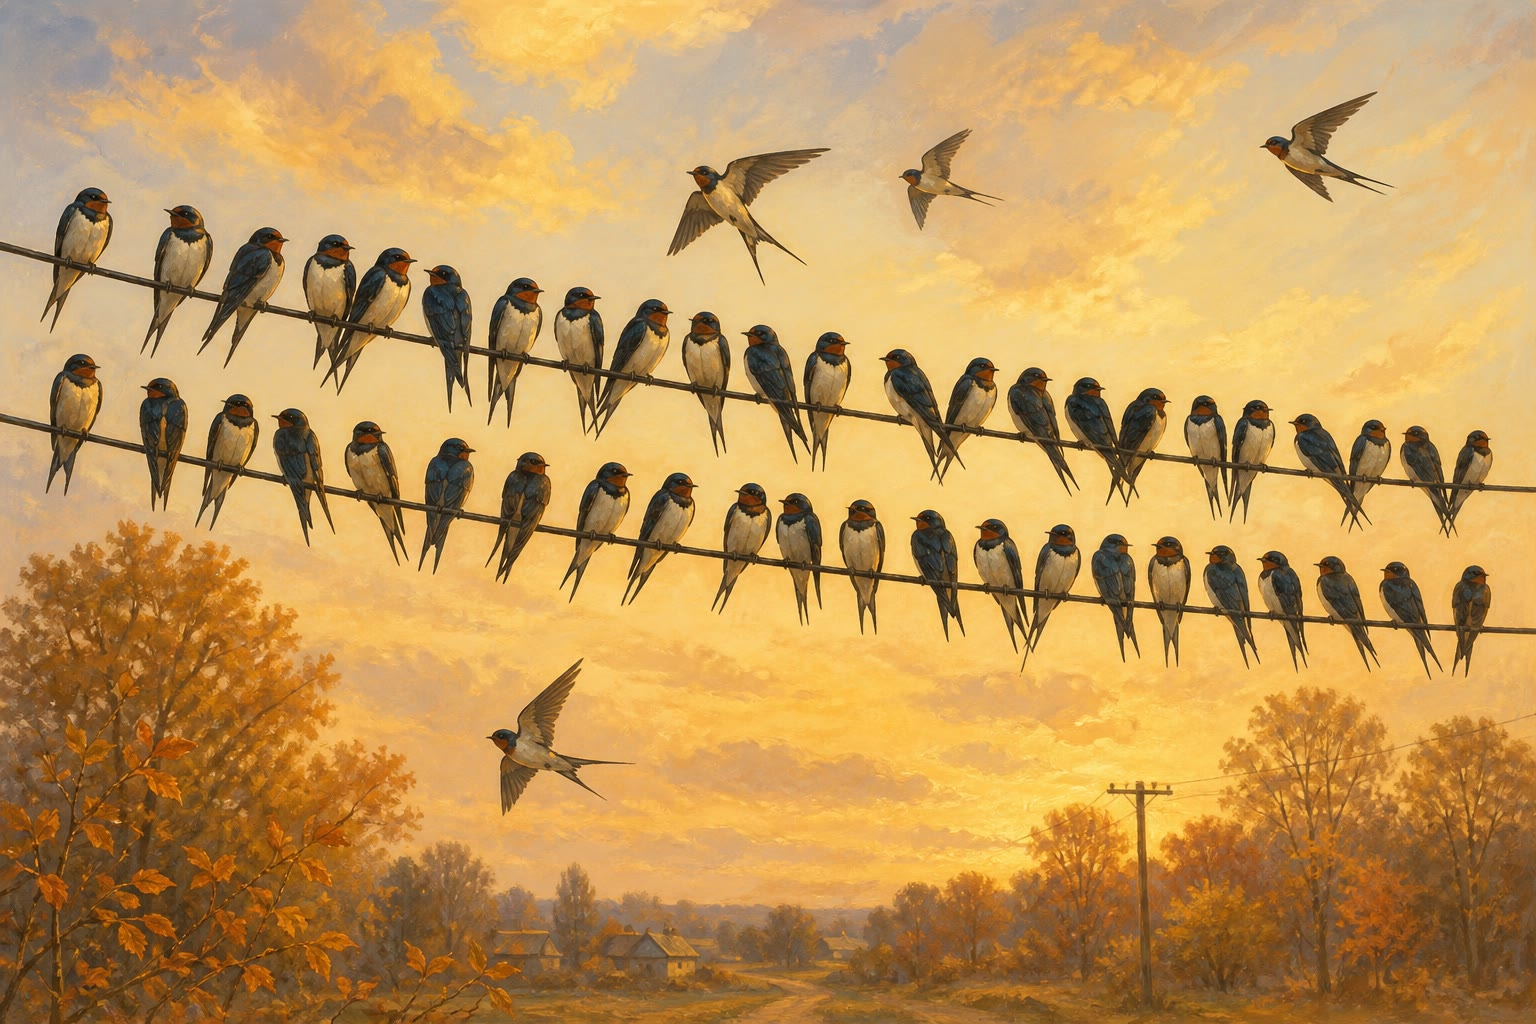
\includegraphics[width=0.62\linewidth]{images/book1/ai/g3-seasons-swallows.jpg}

{\small Bulan Oktober di kawat listrik: \omterm{prop:g3:sorting-living-things:groups}{burung} layang-layang berkumpul
untuk berangkat, beberapa hari sebelum \omterm{prop:g3:sorting-living-things:groups}{serangganya} habis.}
\end{omfigure}

\section{Tiga jawaban atas musim dingin}

\begin{definition}[Migrasi]\label{def:g3:animals-through-seasons:migration}
\emph{Bermigrasi}\index{bermigrasi} berarti mengembara, setiap tahun,
dari satu daerah ke daerah lain seiring pergantian musim ---
berangkat sebelum musim dingin menuju negeri yang lebih hangat tempat
makanan masih ada, lalu kembali pada musim semi. \omterm{prop:g3:sorting-living-things:groups}{Burung} layang-layang,
bangau dan \omterm{prop:g3:sorting-living-things:groups}{burung} jenjang adalah \emph{pemigrasi}\index{migrasi};
sebagian mengembara ribuan kilometer, dan menemukan jalan kembali ke
sarang yang persis sama.
\end{definition}

\begin{definition}[Hibernasi]\label{def:g3:animals-through-seasons:hibernation}
\emph{Berhibernasi}\index{berhibernasi} berarti melewatkan musim
dingin dalam \omterm{prop:g1:healthy-habits:needs}{tidur} yang dalam dan dingin, tersembunyi di sebuah
tempat berlindung: tubuhnya mendingin, jantung dan napasnya melambat
sampai hampir tidak ada, dan \omterm{def:g1:animals-around-us:animal}{hewannya} hidup pelan-pelan dari lemak
yang ditimbunnya pada musim gugur. Landak, tikus \omterm{prop:g1:healthy-habits:needs}{tidur}, marmot gunung
dan kelelawar berhibernasi.
\end{definition}

\begin{definition}[Tetap aktif]\label{def:g3:animals-through-seasons:active}
Sisanya \emph{tetap aktif}\index{tetap aktif pada musim dingin} lalu
mengubah perlengkapan atau kebiasaannya: \emph{mantel musim
dingin}\index{mantel musim dingin} yang lebih tebal,
\emph{cadangan}\index{cadangan makanan} makanan yang dikumpulkan pada
musim gugur (kacang yang dikubur tupai), pergantian daftar makanan
(\omterm{prop:g3:sorting-living-things:groups}{burung} hitam pada \cref{ex:g2:what-animals-eat:winter}), atau sekadar
pencarian yang lebih keras --- rubah, rusa, \omterm{prop:g3:sorting-living-things:groups}{burung} robin.
\end{definition}

\begin{omfigure}
\begin{tikzpicture}
  \draw[thick, omDef, fill=omDef!7, rounded corners=6pt]
    (0,0) rectangle (4.1,3.1);
  \draw[thick, omProp, fill=omProp!7, rounded corners=6pt]
    (4.5,0) rectangle (8.6,3.1);
  \draw[thick, omMeth, fill=omMeth!7, rounded corners=6pt]
    (9.0,0) rectangle (13.1,3.1);
  \node[font=\small\bfseries, omDef, text height=1.6ex, text depth=0.4ex]
    at (2.05,2.75) {bermigrasi};
  \node[font=\small\bfseries, omProp, text height=1.6ex, text depth=0.4ex]
    at (6.55,2.75) {berhibernasi};
  \node[font=\small\bfseries, omMeth, text height=1.6ex, text depth=0.4ex]
    at (11.05,2.75) {tetap aktif};
  \node[font=\small, align=center, text width=3.8cm] at (2.05,1.2)
    {berangkat ke negeri\\ tempat makanan masih ada\\[2pt] layang-layang, bangau,\\ jenjang};
  \node[font=\small, align=center, text width=3.8cm] at (6.55,1.2)
    {tidur dalam yang dingin,\\ hidup dari lemak timbunan\\[2pt] landak, marmot gunung,\\ tikus tidur, kelelawar};
  \node[font=\small, align=center, text width=3.8cm] at (11.05,1.2)
    {mantel musim dingin, cadangan,\\ daftar makanan baru, pencarian keras\\[2pt] rubah, tupai,\\ robin, rusa};
\end{tikzpicture}

{\small Tiga cara melewati musim dingin yang sama. Masing-masing
memecahkan masalah gandanya --- kehangatan dan makanan --- dengan cara
yang berbeda.}
\end{omfigure}

\begin{example}[Tiga tetangga, tiga siasat]\label{ex:g3:animals-through-seasons:three}
Satu pagar tanaman pada bulan Januari: \omterm{prop:g3:sorting-living-things:groups}{burung} layang-layang yang
bersarang di atasnya sedang berada di Afrika, menangkap \omterm{prop:g3:sorting-living-things:groups}{serangga} di
bawah matahari yang hangat; landak di bawahnya \omterm{prop:g1:healthy-habits:needs}{tidur} dingin dan pelan
di dalam sarang \omterm{def:g1:plants-around-us:parts}{daunnya}, membakar lemak bulan Agustus; \omterm{prop:g3:sorting-living-things:groups}{burung} robin di
atasnya, dalam \omterm{def:g1:animals-around-us:covering}{bulu} musim dinginnya yang mengembang, berpatroli
mencari \omterm{prop:g3:flowers-fruits-seeds:transform}{buah} beri yang terakhir. Begitu bulan April tiba, ketiganya
akan sibuk lagi di pagar tanaman yang sama.
\end{example}

\begin{remark}[Tidur bukan kemalasan, mengembara bukan piknik]\label{rem:g3:animals-through-seasons:cost}
Tiap siasat punya harganya. Si \omterm{def:g3:animals-through-seasons:migration}{pemigrasi} menanggung risiko perjalanan
yang melelahkan; si penghibernasi harus mengumpulkan setiap gram lemak
musim dinginnya pada musim gugur --- landak yang terlalu kurus pada
bulan November tidak akan bangun pada musim semi; \omterm{def:g1:animals-around-us:animal}{hewan} yang aktif
bertaruh pada penemuan makanan sepanjang bulan-bulan yang paling
lapar. Musim dingin dibayar di muka, atau di tengah jalan, atau hari
demi hari.
\end{remark}

\begin{method}[Menerka siasat musim dingin seekor hewan]\label{met:g3:animals-through-seasons:guess}
\begin{enumerate}
  \item Tanyakan apa yang dimakannya, dan apakah makanan itu ada di
        sini pada musim dingin;
  \item makanannya lenyap sama sekali (\omterm{prop:g3:sorting-living-things:groups}{serangga} terbang, nektar):
        harapkan \omterm{def:g3:animals-through-seasons:migration}{migrasi} atau hibernasi;
  \item makanannya masih dapat ditemukan (\omterm{def:g2:from-seed-to-plant:seed}{biji}, \omterm{prop:g3:flowers-fruits-seeds:transform}{buah} beri, mangsa):
        harapkan musim dingin yang aktif, barangkali dengan mantel
        yang lebih tebal atau cadangan;
  \item periksa pada musim gugur: menggemuk dan menggali sarang
        menunjuk pada hibernasi; berkumpul dalam kawanan menunjuk pada
        keberangkatan.
\end{enumerate}
\end{method}

\begin{example}[Musim semi membatalkan semuanya]\label{ex:g3:animals-through-seasons:spring}
Pada bulan Maret dan April urutannya berbalik: \omterm{prop:g3:sorting-living-things:groups}{serangga} kembali, para
\omterm{def:g3:animals-through-seasons:migration}{pemigrasi} muncul lagi di sarang lamanya, para penghibernasi terbangun
dalam keadaan kurus dan kelaparan, \omterm{def:g3:animals-through-seasons:active}{mantel musim dingin} ditanggalkan.
Musimnya berputar, dan penanggalan \omterm{def:g1:animals-around-us:animal}{hewan} berputar bersamanya ---
musim gugur berikutnya, \omterm{prop:g3:sorting-living-things:groups}{burung} layang-layang akan berjajar lagi di
kawat listriknya.
\end{example}

\section{Latihan}

\begin{exercise}[$\star$]\label{exo:g3:animals-through-seasons:1}
Masalah ganda apa yang diajukan musim dingin kepada setiap \omterm{def:g1:animals-around-us:animal}{hewan}?
\end{exercise}

\begin{exercise}[$\star$]\label{exo:g3:animals-through-seasons:2}
Sebutkan ketiga siasat musim dingin, dengan dua \omterm{def:g1:animals-around-us:animal}{hewan} untuk masing-masing.
\end{exercise}

\begin{exercise}[$\star$]\label{exo:g3:animals-through-seasons:3}
Apa yang terjadi pada tubuh seekor landak yang \omterm{def:g3:animals-through-seasons:hibernation}{berhibernasi} selama
\omterm{prop:g1:healthy-habits:needs}{tidur} panjangnya? Ia hidup dari apa?
\end{exercise}

\begin{exercise}[$\star$]\label{exo:g3:animals-through-seasons:4}
Mengapa tepatnya \omterm{prop:g3:sorting-living-things:groups}{burung} layang-layang harus pergi --- apa makanannya,
dan apa yang terjadi pada makanan itu di sini pada musim dingin?
\end{exercise}

\begin{exercise}[$\star$]\label{exo:g3:animals-through-seasons:5}
Sebutkan tiga cara seekor \omterm{def:g1:animals-around-us:animal}{hewan} yang aktif melewati musim dingin,
masing-masing dengan \omterm{def:g1:animals-around-us:animal}{hewannya}.
\end{exercise}

\begin{exercise}[$\star$]\label{exo:g3:animals-through-seasons:6}
Berapa harga tiap siasatnya, menurut
\cref{rem:g3:animals-through-seasons:cost}?
\end{exercise}

\begin{exercise}[$\star$]\label{exo:g3:animals-through-seasons:7}
Pada musim gugur, seekor \omterm{def:g1:animals-around-us:animal}{hewan} terlihat makan besar-besaran dan
melapisi sebuah lubang dengan \omterm{def:g1:plants-around-us:parts}{daun} kering. Siasat mana yang sedang
disiapkannya? Langkah mana pada
\cref{met:g3:animals-through-seasons:guess} yang memberitahumu?
\end{exercise}

\begin{exercise}[$\star$]\label{exo:g3:animals-through-seasons:8}
Cobalah: buatlah daftar musim dingin tentang \omterm{prop:g3:sorting-living-things:groups}{burung} yang
sungguh-sungguh kamu lihat di luar selama satu minggu yang dingin.
Adakah \omterm{prop:g3:sorting-living-things:groups}{burung} layang-layang di dalamnya? Burungmu yang mana yang
memilih siasat aktif?
\end{exercise}

\begin{exercise}[$\star\star$]\label{exo:g3:animals-through-seasons:9}
Pakai \cref{met:g3:animals-through-seasons:guess} pada: (a) tupai
(makan kacang dan \omterm{def:g2:from-seed-to-plant:seed}{biji}); (b) \omterm{prop:g3:sorting-living-things:groups}{burung} jenjang (makan katak dan \omterm{prop:g3:sorting-living-things:groups}{serangga}
padang rumput basah). Apa yang mungkin dilakukan masing-masing pada
musim dingin?
\end{exercise}

\begin{exercise}[$\star\star$]\label{exo:g3:animals-through-seasons:10}
Musim gugur yang hangat membuat seekor landak muda tetap terjaga dan
berburu sampai larut, tetapi ia tetap kurus. Mengapa hal ini berbahaya
baginya, menurut \cref{rem:g3:animals-through-seasons:cost}? Apa yang
dilakukan para penyelamat \omterm{def:g1:animals-around-us:animal}{hewan} terhadap landak musim gugur yang
terlalu kurus?
\end{exercise}
